\documentclass[crop, tikz]{standalone}
\usepackage{tikz}

\usetikzlibrary{positioning}

\begin{document}
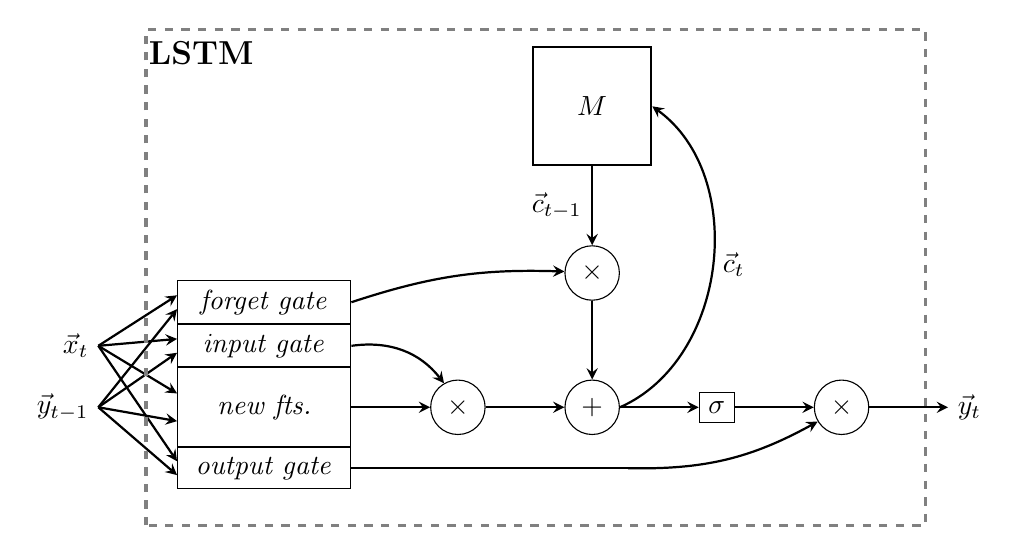
\begin{tikzpicture}
		
	\node[rectangle, draw, minimum width=2.2cm, minimum height=1cm] (FT) {\emph{new fts.}}; 
	\node[rectangle, above =0em of FT, draw, minimum width=2.2cm] (IG) {\emph{input gate}};
	\node[rectangle, above=0em of IG, draw, minimum width=2.2cm] (FG) {\emph{forget gate}};
	\node[rectangle, below=0em of FT, draw, minimum width=2.2cm] (OG) {\emph{output gate}};
	\node[left=of IG] (X) {$\vec{x}_t$};
	\node[left=of FT] (Y) {$\vec{y}_{t-1}$};
		
	\draw[-stealth, thick] (X.east) -- ([yshift=0.5em]FT.west);
	\draw[-stealth, thick] (X.east) -- ([yshift=0.25em]IG.west);
	\draw[-stealth, thick] (X.east) -- ([yshift=0.25em]FG.west);
	\draw[-stealth, thick] (X.east) -- ([yshift=0.25em]OG.west);
	\draw[-stealth, thick] (Y.east) -- ([yshift=-0.5em]FT.west);
	\draw[-stealth, thick] (Y.east) -- ([yshift=-0.25em]IG.west);
	\draw[-stealth, thick] (Y.east) -- ([yshift=-0.25em]FG.west);
	\draw[-stealth, thick] (Y.east) -- ([yshift=-0.25em]OG.west);
		
	\node[circle, draw, right=of FT] (t1) {$\times$};
	\node[circle, draw, right=of t1] (pl) {$+$};
	\node[rectangle, draw, right=of pl] (th) {$\sigma$};
	\node[circle, draw, right=of th] (t2) {$\times$};
	\node[right=of t2] (Y1) {$\vec{y}_t$};
		
	\node[circle, draw, above=of pl] (t3) {$\times$};
		
	\node[rectangle, thick, draw, above=of t3, minimum width=1.5cm, minimum height=1.5cm] (M) {$M$};
		
	\draw[-stealth, thick] (FT) -- (t1);
	\draw[-stealth, thick] (t1) -- (pl);
	\draw[-stealth, thick] (pl) -- (th);
	\draw[-stealth, thick] (th) -- (t2);
	\draw[-stealth, thick] (t2) -- (Y1);
	\draw[-stealth, thick] (M) -- node[left] {$\vec{c}_{t-1}$} (t3);
	\draw[-stealth, thick] (t3) -- (pl);
	\path[-stealth, thick] (IG.east) edge[bend left] (t1);
	\draw[thick] (OG.east) -- ([xshift=10em]OG.east);
	\path[-stealth, thick] (OG.east) -- ([xshift=10em]OG.east) edge[bend right=15] (t2);
	\path[-stealth, thick] (FG.east) edge[bend left=10] (t3);
	\path[-stealth, thick] (pl.east) edge[bend right=60] node[right] {$\vec{c}_t$} (M.east);
		
	\draw[-stealth, very thick, dashed, gray] (-1.5, -1.5) rectangle (8.4, 4.8);
	\node[] (tttxt) at (-0.8, 4.5) {\large \bf LSTM};

\end{tikzpicture}
\end{document}
